\section{Energetic particles in the heliosphere}
\label{sec:particles_heliosphere}

\begin{figure}
	\centering
	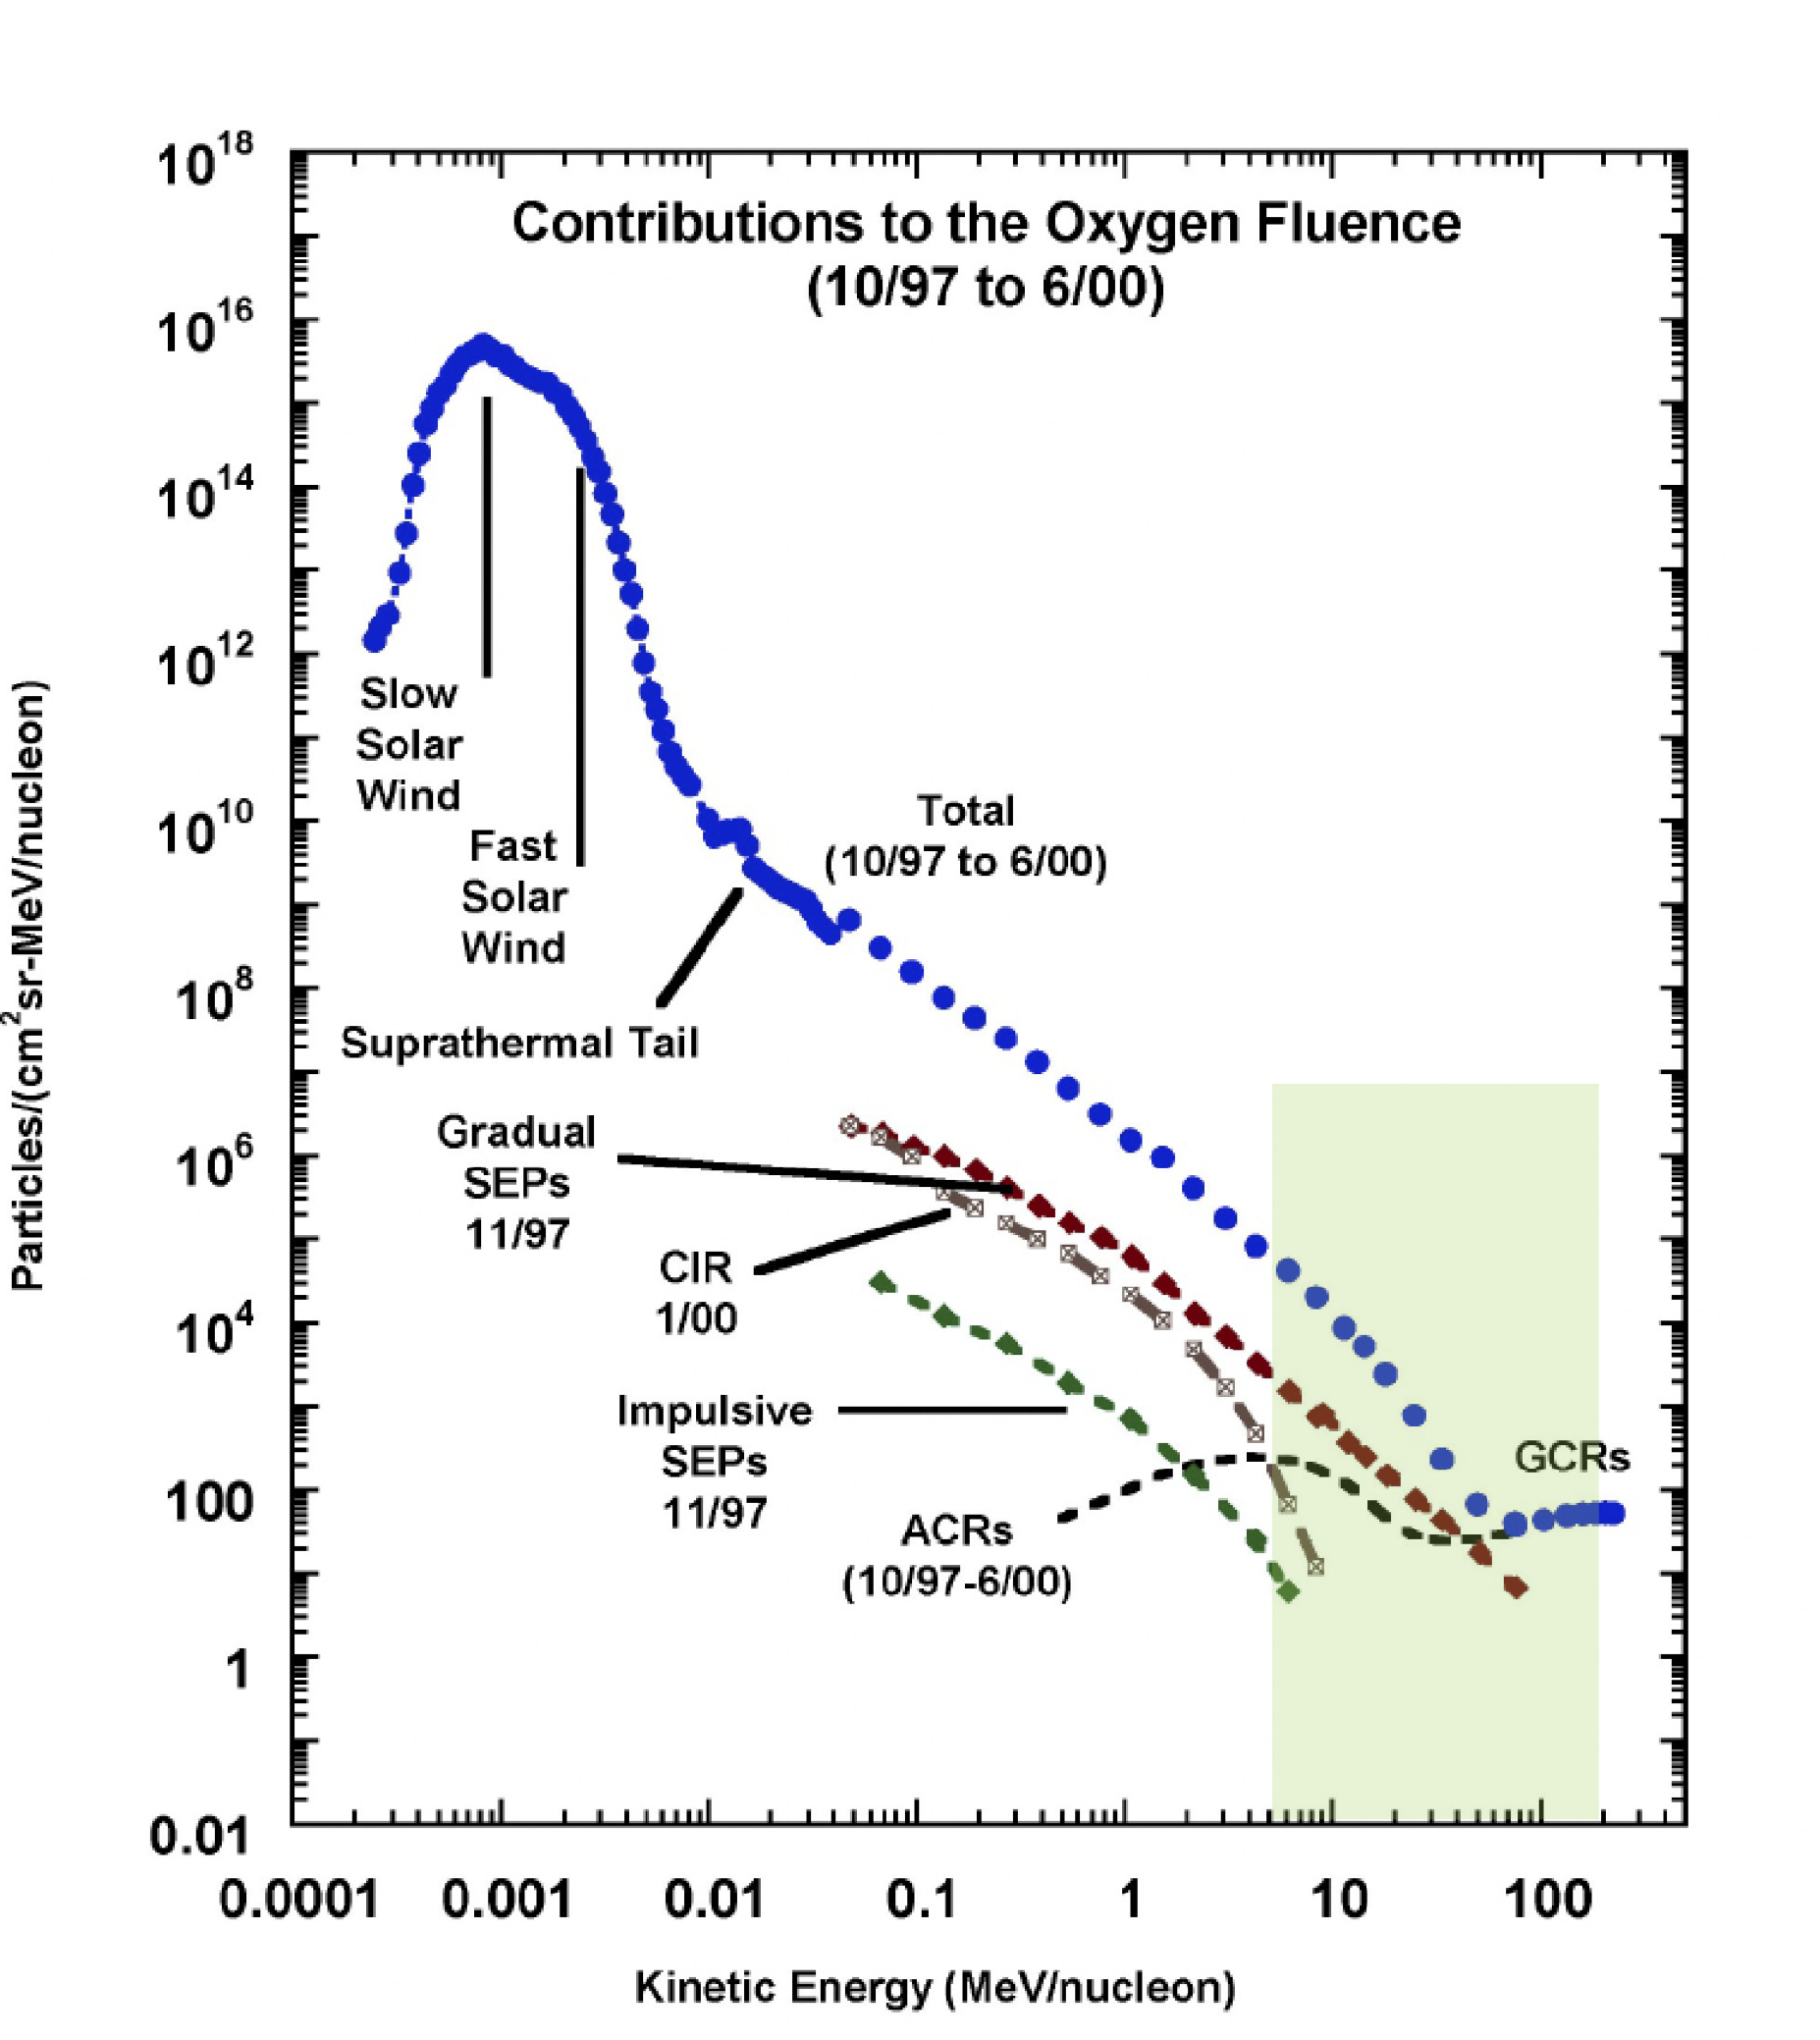
\includegraphics[width = 0.8\textwidth]{images/heliospheric_particle_spectra_color.png}
	\caption[Energy spectra of oxygen ions in near-Earth space]{The typical oxygen spectra in the interplanetary space near Earth, indicating the contributions of different particle populations, particularly in the energy range between few MeV/nuc and few hundreds MeV/nuc (shadow region), where \acs{SEP}, \acs{ACR} and \acs{GCR} coexist. The spectra of other particles species such as, helium and protons have the similar shape but a different flux level in corresponding energy region. The figure is adapted from \citep{Mewaldt-2001}}
	\label{Fig:Oxygen_spectra_heliosphere}
\end{figure}

The heliosphere is a vast, bubble-like region in space that envelops the Sun. This region is moving in the \ac{ISM} with a speed of about 25 km/s \citep{McComas2015ApJS}. Such a cavity is created by the sun and governd by its magnetic field and solar wind; a substantial amount of plasmas of various particle populations fill this space. The particle populations could be identified from Fig.\ref{Fig:Oxygen_spectra_heliosphere} which is adapted from \citet{Mewaldt-2001}. Based on the accumulated measurements of oxygen by the \ac{ACE} between 1997 and 2000 at 1 au, the oxygen fluence spectrum which spans over more than 7 orders of magnitude from keV/nuc to GeV/nuc provides clear insight into the lower energy particles including slow solar wind, fast solar wind, suprathermal tails, and high energetic particles composed of \acp{SEP}, \acp{ACR}, and the extremely high energetic \acp{GCR}. 
Among them \acp{GCR} originate from distant sources outside the solar system, while \acs{ACR} sources are located near the boundary of heliosphere. The remaining energetic particles are accelerated and generated inside of the heliosphere at the multiple locations, including solar surface, interplanetary space and even the planets for instance Jupiter.

The solar wind is a stream of charged particles released from the solar corona, the upper atmosphere of the Sun. This plasam consists of mainly protons and electrons that continously flow outward and expend to about $\sim$ 100 au (depends on direction). The typical energy range of the solar wind is between 0.5 keV and 4.5 keV. Depending on the locations on the sun that produces the solar wind, the speed and density of solar wind might be different. For instance the fast solar wind with a typical speed between 500 and 800 kilemeters per second emits from the coronal holes which are funnel-like regions of open field lines in the magnetic field and usually appear in the north and south pole of sun. Therefore, the fast solar dominate the high latitude regions. While the slow solar wind is observed to have a velocity of about 300 - 500 kilometers per second and is believed to originate from the streamer belt along the equatorial belt. The slow solar wind is more likely to be observed in the low latitude regions.

%plasma embedding with magnetic field

Suprathermal particles are charged ions and electrons that move about two to hundreds times faster than the solar wind particles. In the spectrum shown in Fig.\ref{Fig:Oxygen_spectra_heliosphere}, the suprathermal particles are beyond the tails of the fast solar wind and the dominate particles between few keV to hundreds of keV. The source of suprathermal particle might be the accelerated solar wind and the remanent of the previous solar eruptions and \ac{SEP} events. Those particles play am important role in contributing seed particles for the \ac{SEP} events.

Above the energy of suprathermal particle are the energy range that we are interested in this thesis, especially the energy range between 10 MeV/nuc and few hundred MeV/nuc where the dominated particles are \ac{SEP} (not limited to this energy range),\ac{ACR} (up to $\sim$ 100 MeV/nuc) and lower energy \ac{GCR}. The measurements we used in this study are from this energy range.

The \ac{SEP} are the high energetic particles with energy of few keV up to $\sim$ GeV oriented from the sun and accelerated during the solar activities like solar flare and \ac{CME} driven shocks. \acs{SEP} events are recurring, short term, and intensive. Different type of \acs{SEP} events persist for different time scales from few hours to few days. Such high energy particles are one of the major threats in the space.
%also particle from solar, accelerated by different mechanism. The enery range of \ac{SEP} are quite broad, especially depending the on where the measurement carried on. Recently \ac{SOLO} and \ac{PSP} frequently measure the hundreds keV \ac{SEP}.

\acs{ACR} are believe to be the high energy interstellar pick-up ions \citep{Giacalone2022SSRv} which are ionized neutral interstellar atoms generated by solar UV radiation after they move cross the boundary and enter the heliosphere. Those ionizing particle are then carried by the expanding solar wind to the outer boundary of helioesphere, where they are accelerated by the termination shock and then propagate inwards. The typcial \ac{ACR} species that have been observed are proton, helium, oxygen, nitrogen, iron, neon. 

\ac{GCR} are the fully ionized particles that are accelerated at the so-called supernova remnants \citep{Blasi2013AARv2013} which are outside of the solar system. Those high energy particles bombard Earth in a constant and slowly varying way. The complete GCR spectrum cover the energy from typical 1MeV \citep{Potgieter2013LRSP} to ZeV which is larger than the energy range in Fig.~\ref{Fig:Oxygen_spectra_heliosphere}. The \acs{GCR} is comprised of about 89\% of hydrogen, 10\% of helium, 1\% of heavier ions as well as electron, positron and antiprotons. 

After entering the heliosphere, the transport of both \acp{ACR} and \acp{GCR} are controled by the \ac{HMF}, hence \ac{ACR}'s and \ac{GCR}'s temporal variaton is highly related to the solar activity and solar modulation, which periodically changes in 11 and 22 year periods. 


% LND and SOLO/EPD are new instruments;

% In the helioshphere, 

% Questions:


% 0. Cross calibrate the new data from new instrument; how is the performance of the new instrument? Are they good enough? - To answer this question
% 1. How the widespread SEP generated



\section{Motivition}

The inspiration of this thesis is from the following three aspects:
\begin{itemize}
	\item New mission and new measurements: Over the last few years, several thrilled missions has been successfully launched after extensive preparation, such as \ac{PSP}, \ac{SolO}, \ac{Bepi}, lunar mission like Chang'E series mission, ESA's Jupiter Icy Moons Explorer - Juice, and Chinese missions like CHASE and ASO-S. In this thesis, we focused particularly on the new measurement from \ac{SolO} and \ac{LND}. The former provide the fantastic oppurtunities to study the solar activities in such a close distanc and the latter is the first human mission on the surface of Moon monitoring the radiation environment. The availability of those new observations could enhance our studies of the helioshphere. 
	Once we have the new data from the new instrument, the most fundemental question is how the data looks like in this new instrument. Are they useful? Any new insight shed into the community: validate the instrument performance;
	\item New solar cycle: The recently solar minimum have ended in 2020 before the starting of th new \ac{SC} 25. Many observations haved already implied the unusual characteristics of this solar cycle. It is all known that the recent solar minimum have the most quite solar. The \ac{GCR} flux reached historically high levels in the space age \citep{Fu2021ApJS, Xu2022FrASS}, but ACR intensities did not reach such high, record-setting levels \citet{Strauss2023ApJ}. Moreover, the solar activities raised up rapidly and it could be the strongest \ac{SC} since records begin \citet{Nagovitsyn2023SoPh}. The peak of the solar cycle might arrive 1 year earlier than the prediction \citet{McIntosh2020SoPh}. On the other hand, after the solar minimum, the increasing solar eruptions and \ac{SEP} events provide researchers more oppurtunities to study the solar activities and their impact on the Earth and planet. Question: How the GCR modulated during the solar minimum? what is the drift and diffusion of ACR looks like in the new cycle?

	\item Multipoint observations in the heliosphere: With the increasing number of mission deployed in the space, multipoint observations is becoming more and more important and prevalent, enabling comprehensive moitoring of the solar activities at wide spread regions and at different radial distance. Question: How the wide spread event look like? Any discrepancy between the observation from SOLO and other instruments.
	
\end{itemize}


Therefore, following the idea of utilizing the new measurements from \ac{SolO} and \ac{LND}, in this thesis, we presents the first  observations of \ac{SEP} from \ac{LND} in Sec.~\ref{chp:LND_SEP}, \ac{GCR} and secondary proton measured on the lunar surface in Sec.~\ref{chp:LND_GCR_albedo}, quite time spectra (\ac{GCR}) measured in the inner heliosphere(Sec.~\ref{chp:SOLO_Quite_time})and the change of the \ac{ACR} helium radial gradient in the new solar cycles (Sec.\ref{chp:ACR_Helium}).
The introduction of the instrument \ac{LND} and \ac{SolO}/\ac{HET} is given in Sec.~.\ref{chp:instruments}. The summary and outlook conclude this thesis. In particular, more detailed information of the \ac{LND} are provided in the Appendix ~\ref{chp:LNDinstrument}

% The exploration of space has witnessed a surge in intensity, with an increasing number of countries aspiring to venture into this domain. Noteworthy examples include NASA's initiation of the Artemis mission, which aims to return to the Moon by 2024. Similarly, China has unveiled its plans to establish a lunar base on the lunar surface by the 2030s, while the European Space Agency (ESA) has also embarked on a lunar lander mission. Most recently, a Japanese lunar lander mission was launched; however, it regrettably encountered failure.

% Under these circumstances, the study of solar energetic particles (SEPs) assumes greater significance. SEPs pose a significant radiation hazard for future human exploration on the lunar surface. The most hazardous SEP events have the potential to induce radiation increases of substantial magnitude.

% SEP events directed towards Earth can become an issue of space weather and
% very energetic events can cause a so-called Ground Level Enhancement (GLE).
% This means that the radiation level on the ground increases which can be seen in
% neutron monitor measurements.